%%%%%%%%%%%%%%%%%%%%%%%%%%%%%%%%%%%%%%%%%%%%%%%%%%%%%%%%%%%%%%%%%%%%%%%%%%%%%
%%
%% This file provides a template that can be used in concert with the
%% ohio-etd class to generate an electronic thesis or dissertation which
%% meets the formatting requirements at Ohio University.
%%
%% To use the template, copy this file (template.tex) and ohio-etd.cls into
%% the same directory and edit this template as required.  Reference
%% ohio-etd.pdf for additional instructions on using this class.
%%
%%%%%%%%%%%%%%%%%%%%%%%%%%%%%%%%%%%%%%%%%%%%%%%%%%%%%%%%%%%%%%%%%%%%%%%%%%%%%


%% Load the class.  Available options are: numbered, pdftex, cmfont,
%% singlespacetables, draft, 11pt, 12pt, leqno, and fleqn

\documentclass[numbered,pdftex]{ohio-etd}
\usepackage{cite}
\usepackage{notoccite}

\usepackage{ragged2e}
\usepackage{verbatim} 
\usepackage{hyperref}
\usepackage{flafter}
\usepackage{color,soul} % Highlighting 
\usepackage{subfigmat}

\usepackage{float} % In-text figs
\usepackage{varioref}%  smart page, figure, table, and equation ref
\usepackage{graphicx} % Include graphics
\usepackage{epstopdf} % Figure type .eps to .pdf
\usepackage{wrapfig} % Figures in text
\usepackage{listings}
\usepackage{color} %red, green, blue, yellow, cyan, magenta, black, white
\definecolor{mygreen}{RGB}{28,172,0} % color values Red, Green, Blue
\definecolor{mylilas}{RGB}{170,55,241}
%% Other packages that may be of use.  Delete or comment out (using a
%% percent sign in the first column) if they are not desired.  Reference
%% the corresponding documentation for more information on how to use these
%% packages.

%\usepackage[square,sort&compress,numbers]{natbib} % Provides formatting for
                                                  % citations
\usepackage{textcomp} % Provides math symbols that can be used in text mode
\usepackage{amssymb}  % Provides additional AMS math symbols.  Note that
                      % amsmath is loaded as part of the ohio-etd class
\usepackage{bm}       % Provides bold-faced math symbols
\usepackage{booktabs} % Provides improved table formatting
\usepackage{dcolumn}  % Provides table columns aligned at decimal points
\usepackage{multirow} % Provides table elements spanning multiple rows
\usepackage{graphicx} % Standard package to incorporate graphics
\usepackage[printonlyused]{acronym} % Provides a method for incorporating
                                    % acronyms and building an acronym list
\usepackage{relsize}
\usepackage{amsmath} % Inserting Equations

\graphicspath{{figures/}} % Allows graphics files to be stored in a
                          % separate directory
\usepackage{fancyref}
\usepackage{}

%% Required front matter definitions

\degree    {MS}              % MS, MA, MCTP, or PhD
\graduation{December}{2017}    % May, August, or December 

\title     {A Proposal for a Parameterized Circulating Vector Field Guidance for Fixed Wing Unmanned Aerial Vehicles}
\author    {Garrett S.}{Clem} 

\advisor   {Jay P. Wilhelm}{Assistant Professor of Mechanical Engineering}
\dean      {Dennis Irwin}{Dean, Russ College of Engineering and Technology }
\program   {Mechanical Engineering}            % e.g. Electrical Engineering
\department{Department of Mechanical Engineering} % e.g. School of Electrical Engineering 
                                    %      and Computer Science
\college   {Russ College of Engineering and Technology}   % e.g. Russ College of Engineering and
                                     %      Technology
\abstract  {ABSTRACT}


%% Optional front matter definitions.  Delete or comment out if not needed

% \coadvisor {Coadvisor's Full Name}{Coadvisor's Full Title}

\dedication{DED}

\acknowledgments{ACK}
%% If you prefer to provide "acknowledgements" instead (note the added "e"
%% between the "g" and the "m") then add the "e" in the macro name so that
%% it reads "\acknowledgements".}

%% Additional "lists" can be added to the end of the front matter using the
%% \addlistof macro.  For example:
\addlistof{Symbols}{\begin{tabbing}
  XXXX \= \kill% this line sets tab stop
  \\
  $a$ \> Previous or Initial Axial Induction Factor (-) \\
  

 \end{tabbing}}
%% Note that the command "\input{symbols}" can be used if the symbol list is
%% contained in a separate file called "symbols.tex"}

\addlistof{Acronyms}{

\begin{tabular}{lll}
AoA & Angle of Attack & \\
\end{tabular}}


%% Use "\input{acronyms}" if the acronym list is in a separate file called
%% "acronyms.tex".  Note that the formatting generated by the acronym package
%% can be forced into singlespaced text by inserting "\setlength\itemsep{0pt}
%% \setlength\parskip{0pt}" into the "acronym" environment.} 

%% For documents created by government employees as part of their
%% employment.  The wording of the disclaimer can be specified using an
%% option.  See the documentation for more information.

% \govtdisclaimer    

% \notables  % Prevent a list of tables from being created
% \nofigures % Prevent a list of figures from being created

\begin{document}

\makefrontmatter    % Creates all of the front matter pages.

% for matlab code entrys
\lstset{language=Matlab,%
    %basicstyle=\color{red},
    breaklines=true,%
    morekeywords={matlab2tikz},
    keywordstyle=\color{blue},%
    morekeywords=[2]{1}, keywordstyle=[2]{\color{black}},
    identifierstyle=\color{black},%
    stringstyle=\color{mylilas},
    commentstyle=\color{mygreen},%
    showstringspaces=false,%without this there will be a symbol in the places where there is a space
%     numbers=left,%
%     numberstyle={\tiny \color{black}},% size of the numbers
%     numbersep=6pt, % this defines how far the numbers are from the text
    emph=[1]{for,end,break},emphstyle=[1]\color{red}, %some words to emphasise
    %emph=[2]{word1,word2}, emphstyle=[2]{style},    
}

%% Body of the text follows, using \chapter, \section, \subsection,
%% \subsubsection, \paragraph, and \subparagraph to generate the
%% section headings.  For convenience, it may be useful to break the
%% full document into separate files, perhaps divided by chapters.  In
%% that case, the files would be loaded here using "\input{filename}"


\chapter{Introduction}
\section{Motivation and Problem Statement}

%Fixed wing Unmanned Aerial Vehicles are used for missions such as surveillance and reconnaissance that might put pilots harm’s way \cite{bone_uavs_2003}. Missions consist of sequential objectives that are represented by a path that the UAV attempts to follow. Paths are typically pre-planned before flight and are constructed by connecting straight lines and circular arcs. Vehicle turn rate constraints and obstacles are considered when planning a path to prevent collisions or entry into no-fly zones. UAVs are guided to follow a path by implementing guidance algorithms which calculate headings that minimize the distance to a path. UAVs may encounter an obstacle whose position was previously unknown while following a pre-planned path which may require a new path to be generated. Guidance that follows mission paths while avoiding obstacles without the need for re-planning may be beneficial. 
%\\
%Gradient Vector Field (GVF) guidance is a path following method that has been adapted for obstacle avoidance. GVFs produces continuous heading vectors that guide a UAV to converge and follow a path by summing together convergence and circulating terms that are weighted by static scalars. An obstacle represented as a path and given a negative convergence weight results in a repulsive field that can be used for obstacle avoidance. Static GVFs do not always route the UAV around an obstacle and could be improved. Modifying the GVF convergence and circulation weights of obstacle fields to be functions of common UAV states could be used to produce an optimal guidance for obstacle avoidance. \textbf{The proposed research seeks to determine GVF weighting functions that construct optimal obstacle avoidance.}
Fixed wing Unmanned Aerial Vehicles (UAVs) are used for missions such as surveillance and reconnaissance that might put pilots in harm’s way \cite{bone_uavs_2003}. Missions typically consist of sequential objectives represented as waypoints that the UAV follows. Waypoints may be pre-planned before flight where vehicle constraints and obstacles can be considered to prevent collisions or entry into no-fly zones. UAVs follow waypoints by implementing guidance algorithms that calculate headings that direct the UAV along a path connecting the waypoints. Obstacles may be discovered during flight that were unknown at initial planning and a new set of waypoints may have to be generated.  Waypoints are typically computed at a ground station and are relayed to the UAV by radio, which may be problematic if communication with the UAV is lost. Guidance that accomplishes mission objectives while avoiding obstacles without the need for re-planning waypoints may be beneficial. 
\\
Vector Field (VF) guidance is a method that is mainly used for path following and can be useful for obstacle avoidance [W,W,C]. VFs can produce continuous heading vectors that can be used guide a UAV to coverage and follow a path. Vectors are calculated by summing together convergence and circulation terms that are weighted by static scalars. Obstacles can be represented as a path and given a negative convergence weight resulting in a repulsive field. Static repulsive VFs do not always route the UAV around an obstacle. Modifying repulsive VF parameters to be functions of common UAV states could be used to produce an optimal guidance. \textbf{The proposed research seeks to determine VF weighting functions that enable optimal obstacle avoidance.}



 \pagebreak
 
 





\chapter{Literature Review}
\section{Introduction to Literature Review}


\section{Unmanned Aerial Vehicle}

Unmanned Aerial Vehicles (UAVs) are pilotless aircraft used by military, police, and civilian communities for tasks such as surveillance, reconnaissance, damage assessment, and natural disaster surveying.  UAVs are generally categorized into fixed wing and rotor craft varieties that range in size, payload, and flight time capabilities. The aircrafts can be controlled remotely with a RC transmitter or fly on paths connecting pre-planned waypoints. Data can be collected with on-board sensors, such as cameras, which can be stored or relayed to the ground. UAVs are part of an Unmanned Aerial System (UAS) which is made up of the vehicle, autopilot, ground station, transmitter, and two way radio, depicted in Figure \ref{fig:uas}. Ground stations are responsible for monitoring the vehicle's status, planning missions, and generating obstacle free and flyable paths which are sent to the autopilot via two way radio. 

\begin{figure}
	\centering
	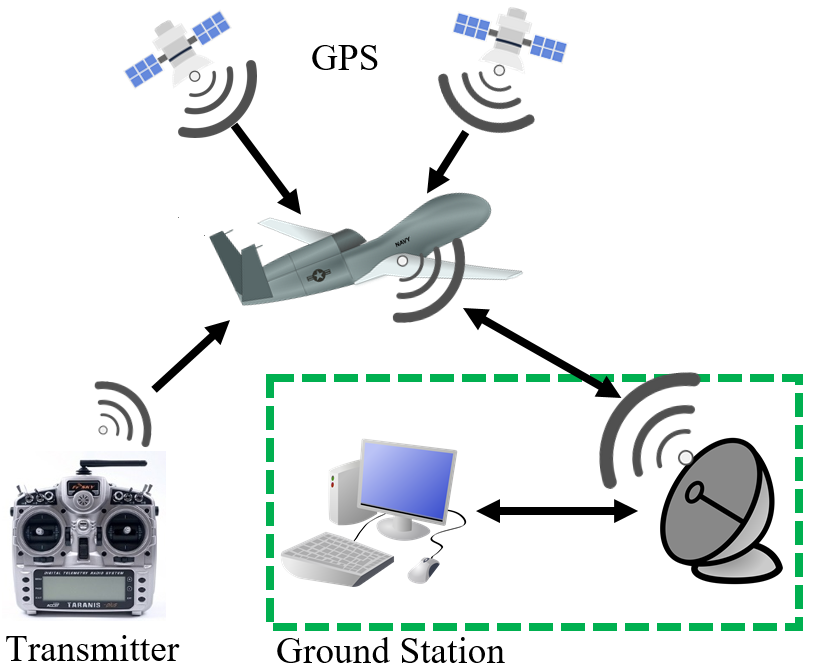
\includegraphics[width=8cm]{PaperFigures/UAS}
	\caption{Unmanned Aerial System (UAS)}
	\label{fig:uas}
\end{figure}

The autopilot is responsible for following a pre-planned path and maintaining vehicle stability while under the influence of external wind disturbances. Stable flight while path following is accomplished by implementing feed-back control, navigation, and guidance systems. Feed-back refers to the closure of an open-loop control system which allows an error to be calculated between the desired state of the UAV, the reference, and the current state of the UAV. Reference error is used to calculate the necessary actuator output required to modify the vehicles attitude and position while preventing unbounded osculations. Feed-back is provided by the navigation system which uses sensors to measure the attitude and position of the aircraft. Sensors often provide noisy data and are sampled at varying rates. Filtering and estimation techniques such as the Kalman filter which fuses and filters measurements to provide an improved state estimation. A high level overview of the autopilots systems can be seen in Figure \ref{fig:autopilotloops}.

\begin{figure}
	\centering
	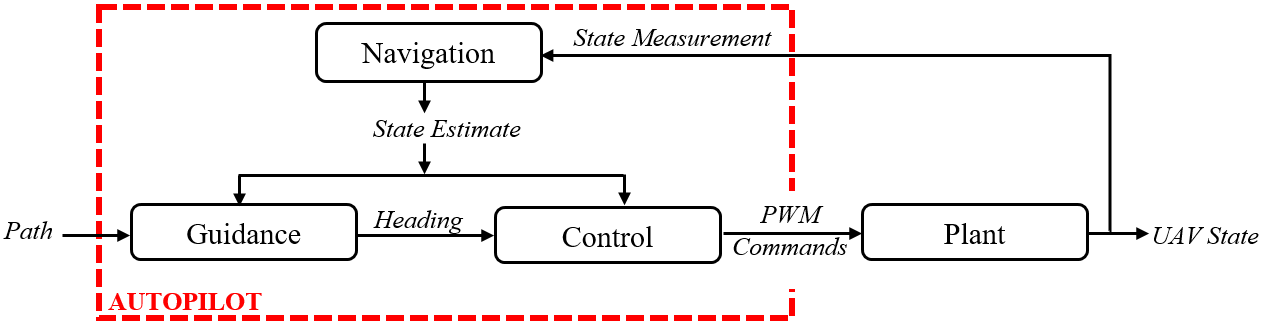
\includegraphics[width=15cm]{PaperFigures/autopilotLoops}
	\caption{Autopilot's Navigation, Guidance, and Control Architecture}
	\label{fig:autopilotloops}
\end{figure}

The navigation system is responsible for taking high level pre-planned paths from the ground station and providing a reference heading command to the control system. Several methods for path following guidance were investigated in \cite{sujit_unmanned_2014} consisting of carrot chasing, non-linear guidance law, pure line-of-sight, linear quadratic regulator, and gradient vector field method. A Monte Carlo simulation with wind disturbances was conducted for the guidance methods above in \cite{sujit_unmanned_2014}. It was determined that the vector field method followed the path with least tracking error and control effort which is the primary goal of path following. 


\section{Vector Field Guidance}
\subsection{Introduction to Vector Field Guidance}
 Vector Field is a computationally inexpensive guidance and control approach that can be used to transition a robotic system from an initial state to a goal state. Goals act as artificial attractive forces that pull on the robotic system while obstacles act as artificial repulsive forces that push the robotic system away. Classes of vector fields can be categorized as singular or path following algorithms. Potential Field and Virtual Force Field (VFF) methods converge to a single point and avoid obstacles by applying artificial attractive and repulsive forces. Lyapunov and Gradient Vector Fields provide guidance that asymptotically converges to path. Obstacle avoidance has been achieved with Gradient Vector Fields by assigning repulsive weights to a convergence term. Weights currently act as a high level specification of the desired guidance behavior and may be further optimized. 

\subsection{Potential Field}
Potential field models a robots workspace as a gradient potential of attractive and repulsive artificial forces \cite{khatib_real-time_1986}. Robots can be represented as a point mass initially located at a globally maximum potential that transitions to a goal located at a globally minimum potential. Obstacles are represented by a high potential that act as repulsive forces with an exponentially decaying strength as to only influence the robot when approaching the obstacle. The potential gradient can be depicted as a mesh such as that shown in Figure \ref{fig:pfobstacle}. Potential field is unique in that it combines path planning, trajectory planning, and control into a single system \cite{rimon_exact_1992}. 

\begin{figure}[h!]
	\centering
	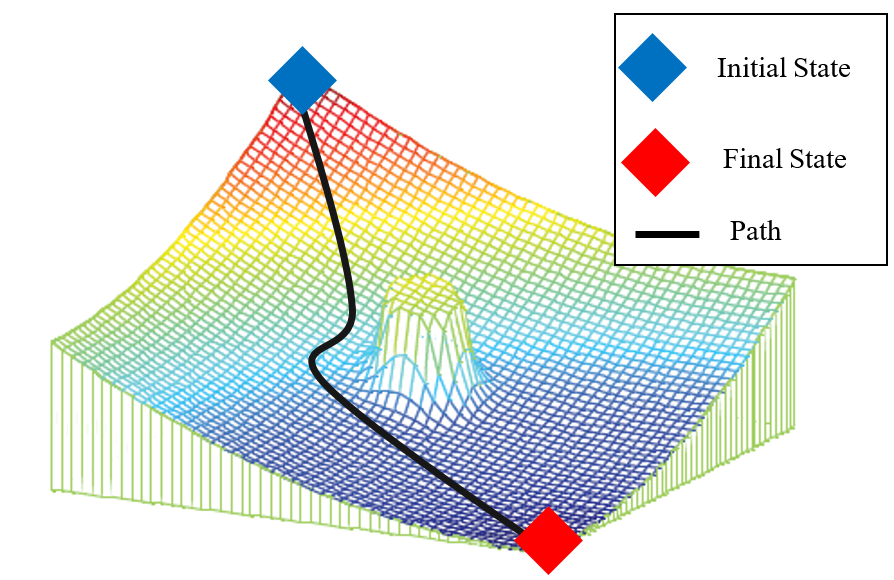
\includegraphics[width=7cm]{PaperFigures/pfObstacle}
	\caption{Single Obstacle Potential Field Gradient \cite{liu_virtual-waypoint_2016}}
	\label{fig:pfobstacle}
\end{figure}


Inherent problems with potential field methods were identified when experimentally validating the Virtual Force Field (VFF) method in \cite{koren_potential_1991}, including local minimums and osculations. VFF operates on the artificial  attractive and repulsive force principle and is intended specifically for mobile robots seeking a goal in an environment with initially unknown obstacles. VFF decomposes a robots workspace into discretized cells that contain an integer certainty value associated with the confidence that an obstacle occupies the cell. A global goal applies an artificial attractive force on the robot that pulls it closer to the goal. As the robot detects obstacle's, the certainty value increases in the cell associated with the obstacles position. Cells apply artificial repulsive forces with magnitudes that depend on the certainty value and the distance to the cell.


\begin{figure}[H]
	\centering
	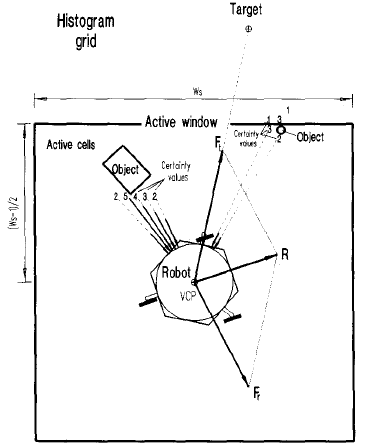
\includegraphics[width=7cm]{PaperFigures/histogram}
	\caption{Virtual force field histogram acting on a mobile robot \cite{borenstein_vector_1991}}
	\label{fig:histogram}
\end{figure}

The VFF histogram method was validated on a mobile robot platform using ultrasonic sensors in \cite{borenstein_real-time_1990} and \cite{borenstein_vector_1991}, avoiding obstacles and seeking a goal. Several problems inherent to all potential field methods were identified while validating the VFF histogram method.  Local minimum produced by closely spaced obstacles may create a situation where a robot settles into a lower potential prior to finding the global minimum which is shown in Figure \ref{fig:pfLocalMin}. Additionally, closely spaced obstacles may also be difficult to pass between, shown in Figure \ref{fig:vff}a. Oscillations can also be experienced near obstacles or in narrow passages at high speeds, shown in Figure \ref{fig:vff}b. 

\begin{figure}[H]
	\begin{subfigmatrix}{2}% number of columns
		\centering
		\subfigure []{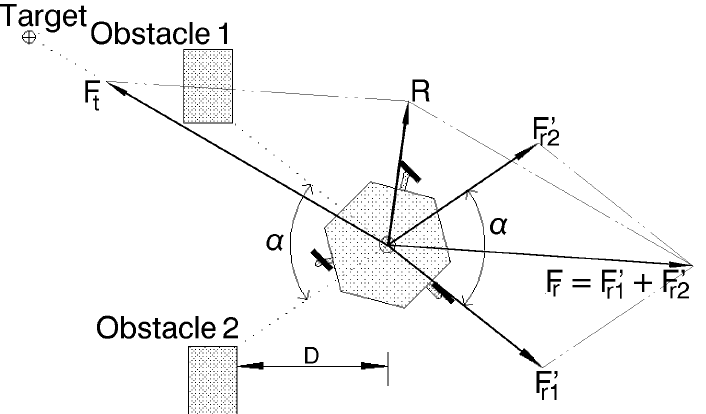
\includegraphics[width=9cm] {PaperFigures/multipleObsVff}}
		\subfigure []{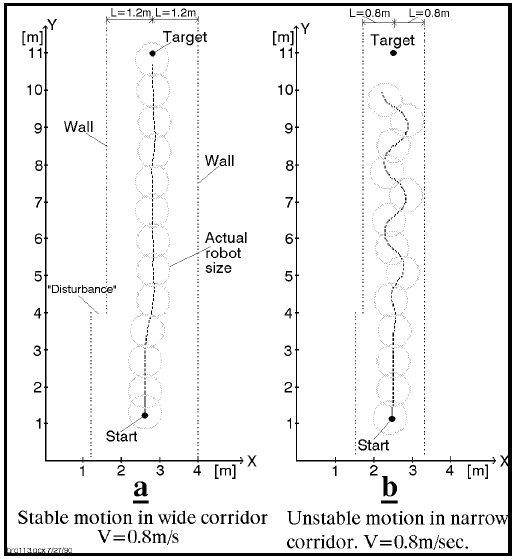
\includegraphics[width=6cm] {PaperFigures/unstableCooridorMotionVff}}
	\end{subfigmatrix}
	\caption{Potential Field Local Minimum \cite{liu_virtual-waypoint_2016}}
	\label{fig:vff}
\end{figure}


\begin{figure}[H]
	\begin{subfigmatrix}{2}% number of columns
		\centering
		\subfigure []{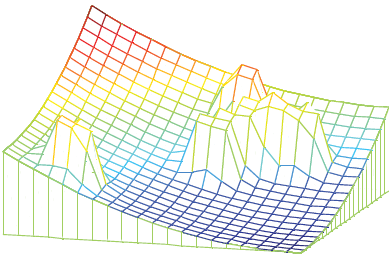
\includegraphics[width=7cm] {PaperFigures/pfObstacleLocalMin}}
		\subfigure []{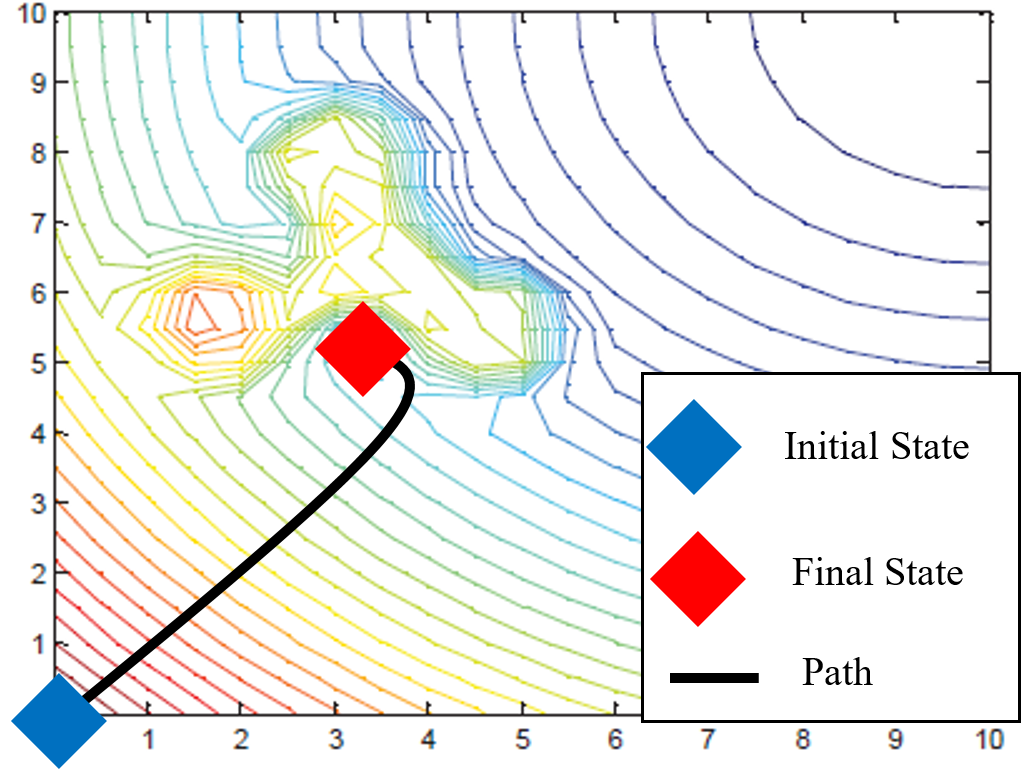
\includegraphics[width=7cm] {PaperFigures/pfObstacleLocalMinTopology}}
	\end{subfigmatrix}
	\caption{Potential Field Local Minimum \cite{liu_virtual-waypoint_2016}}
	\label{fig:pfLocalMin}
\end{figure}


Several methods have been developed to eliminate local minimums of potential fields through the use of navigation functions \cite{goerzen_survey_2010} and obstacle clustering \cite{liu_virtual-waypoint_2016}. Navigation functions relate kinematic constraints to the gradient potential to produce a bounded and local minimum free solution \cite{rimon_exact_1992}. Clustering closely spaced obstacles into a single and equally repulsive obstacle prevents local minimum from forming. Typical clustering can be seen in Figure \ref{fig:obstacleclustering}. 

\begin{figure}[H]
	\centering
	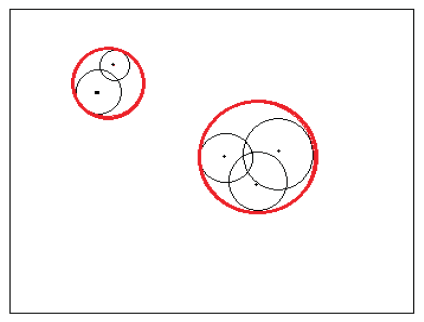
\includegraphics[width=5cm]{PaperFigures/obstacleClustering}
	\caption{Obstacle Clustering \cite{liu_virtual-waypoint_2016}}
	\label{fig:obstacleclustering}
\end{figure}

Potential Field's ability to avoid obstacles and combine path planning, trajectory planning, and control into a single computationally inexpensive system makes it an attractive motion control system for robots seeking a singular point, even with the limitations discussed in \cite{koren_potential_1991}. Unlike ground mobile robots, fixed wing UAVs must maintain a minimum forward velocity and cannot converge to a single point. Vector fields that direct a UAV to paths connecting waypoints have been developed using Lyapunov and gradient vector field techniques. 
 
 
\subsection{Lyapunov Vector Fields}
Lyapunov vector fields produce heading guidance that asymptotically converges and circulates along a path passing through waypoints. Paths can be built from straight line and circular arc primitives taking UAV dynamic constraints into consideration. Vector Fields that guide to straight line and circular paths was introduced in \cite{nelson_cooperative_2005}. Farther away from the path, vectors are constant and point in the direction perpendicular to the path. Within a transition region the vectors begin to rotate and point more parallel to the path. Vectors on the path point directly in the direction of the path. Lyapunov vector fields for straight line and circular arcs are shown in Figure \ref{fig:nelsonlyapunov}.
\begin{figure}
	\centering
	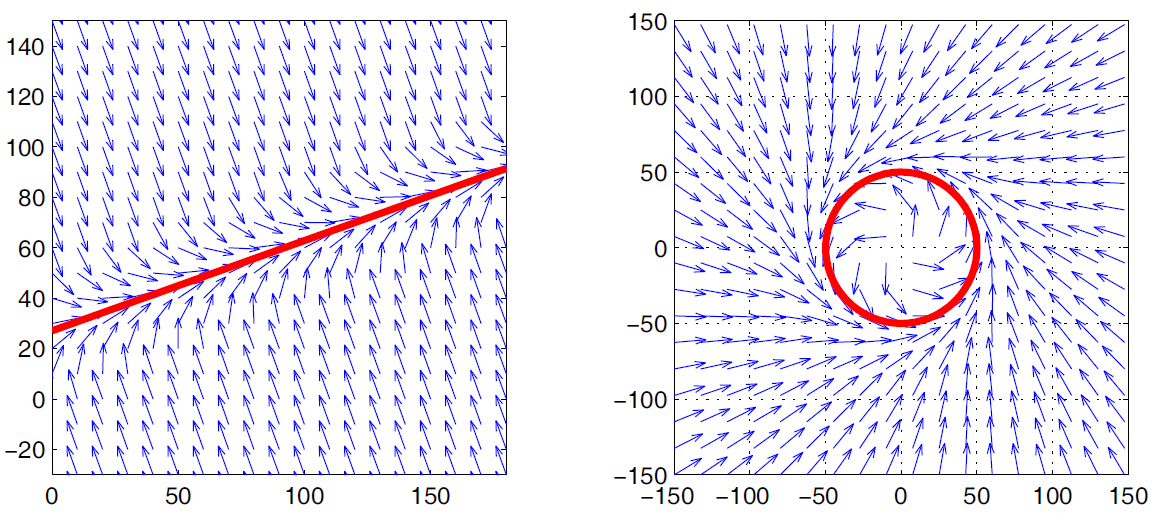
\includegraphics[width=13cm]{PaperFigures/nelsonLyapunov}
	\caption{Lyapunov vector field for straight line and circular primitives \cite{nelson_cooperative_2005}}
	\label{fig:nelsonlyapunov}
\end{figure}

Combining path primitives together can result in fairly complex paths such as that shown in Figure \ref{fig:urbanfollowingnelson}. Each path primitive has a vector field associated with it and determining which field to use can be approached in two different ways. Fields from all of the primitives can be summed together similar to the attractive and repulsive forces in potential field. Second, fields can be selectively activated and deactivated based on the position of the UAV. Summing together vector fields, as pointed out in \cite{nelson_cooperative_2005}, can result in several problems including dead zones, sinks, and singularities. Selectively activating each vector field as a UAV nears waypoints was used in \cite{nelson_cooperative_2005,nelson_vector_2006,nelson_vector_2007}.

\begin{figure}[H]
	\centering
	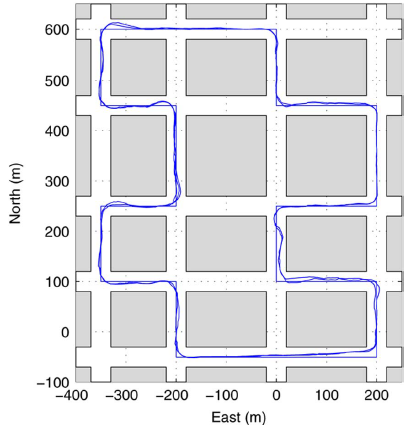
\includegraphics[width=7cm]{PaperFigures/urbanFollowingNelson}
	\caption{Straight path following in urban environment \cite{nelson_cooperative_2005 using} Lyapunov Vector Field}
	\label{fig:urbanfollowingnelson}
\end{figure}


Nelson's method was extended by Griffiths for curved path following and showed that the vectors asymptotically approach the curved path \cite{griffiths_vector_2006}, shown in Figure \ref{fig:griffiths}. Constructing a vector field for an arbitrary curve in place of stitching together primitives has the advantage of not determining which field to activate and may allow for more complex paths.

\begin{figure}[H]
	\centering
	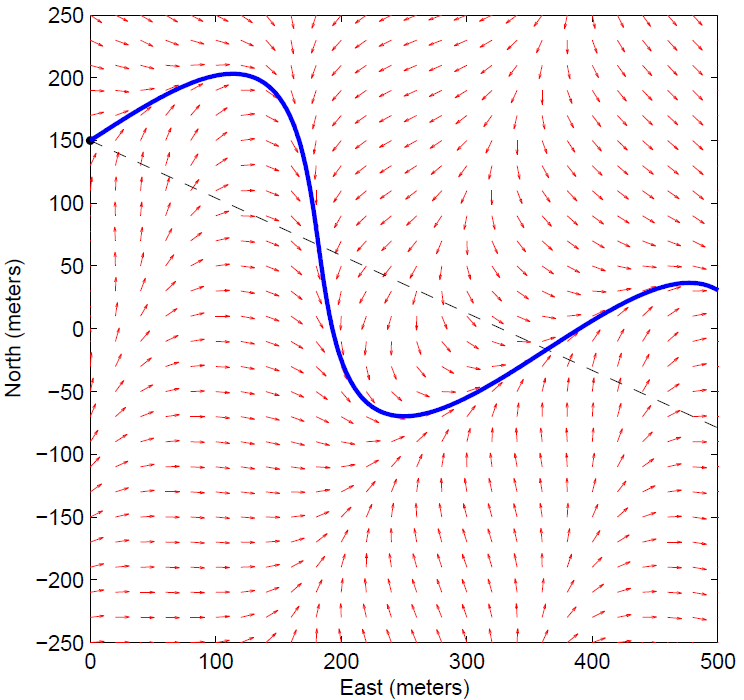
\includegraphics[width=7cm]{PaperFigures/griffiths}
	\caption{Lyapunov vector field approach curved path asymptotically \cite{griffiths_vector_2006}}
	\label{fig:griffiths}
\end{figure}


Primitive circular fields can be modified via non-linear coordinate transformations to produce globally convergent elliptical fields \cite{frew_lyapunov_nodate,frew_cooperative_2007}. Frew simulated and experimentally validated the transformed vector field where multiple fixed wing UAVs cooperatively tracked a moving target while maintaining a staggered distance from each other, preventing collision and multiple surveillance angles. The location of a target being tracked is not known with absolute certainty. The covariance matrix from a kalman filter to transform a circular vector field around an uncertain target was investigated in \cite{frew_cooperative_2007} and an example field is shown in Figure \ref{fig:lyapunovFrew}b.

\begin{figure}[h]
	\begin{subfigmatrix}{2}% number of columns
		\centering
		\subfigure []{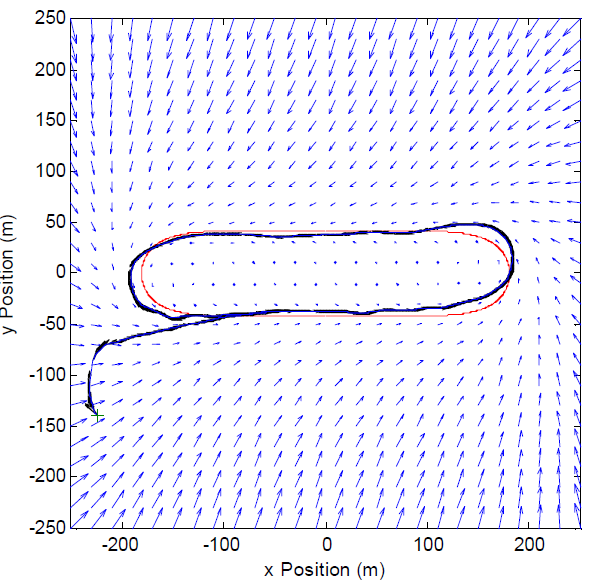
\includegraphics[width=6.25cm] {PaperFigures/lyapunovFrew}}
		\subfigure []{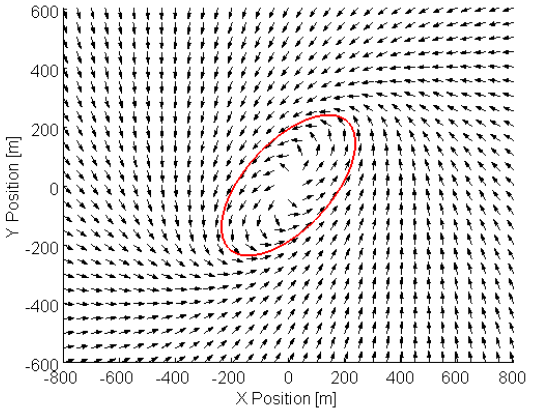
\includegraphics[width=8cm] {PaperFigures/lyapunovFrewUncertain}}
		%		\hspace*{1cm}
	\end{subfigmatrix}
	\caption{Elliptical VF produced by non-linear coordinate transformations a)\cite{frew_lyapunov_nodate} b)\cite{frew_cooperative_2007}}
	\label{fig:lyapunovFrew}
\end{figure}

Target tracking Lyapunov Plus Tangent Vector Field (TPVLF) was introduced in \cite{chen_tracking_2009} that produced shorter paths compared to Lyapunov alone. Outside of the standoff circle, tangent vectors were provided the shortest distance to the circle. Inside the standoff circle, no tangent lines exist and Lyapunov is used in its place. Figure \ref{fig:lyapunovChen} shows the difference in paths taken for Lyapunov and tangent vector fields outside the standoff circle. The TPLVF was later used for path planning to avoid obstacles in \cite{chen_uav_2013}.

\begin{figure}
	\centering
	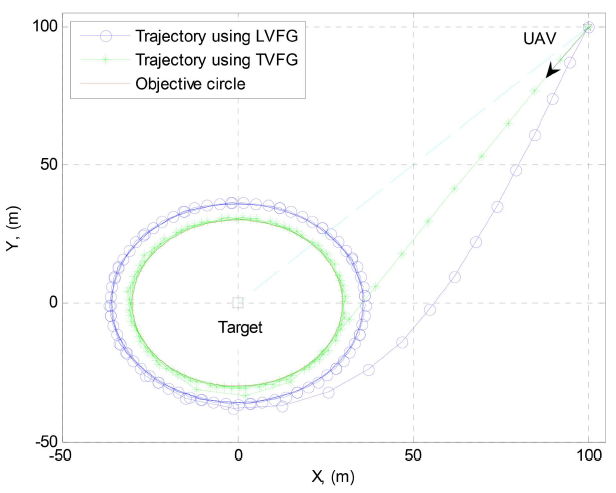
\includegraphics[width=7cm]{PaperFigures/lyapunovChen}
	\caption{Tangent plus lyapunov vector fields for shortest path target tracking \cite{chen_uav_2013}}
	\label{fig:lyapunovChen}
\end{figure}


\subsection{Non-Lyapunov Vector Fields}
All methods that consider obstacles thus far built a vector field that guides the UAV to an obstacle free path. Another approach is to build a vector field tending to a path and use optimal rapid random trees (RRT*) to explore the space for obstacles and select the optimal path \cite{pereira_framework_2016}. Branches extend from the root, or initial location of the UAV, randomly throughout the map with a constrained deviation from the initial vector field. When a branch encounters an obstacle it is trimmed and no longer explored. The path of minimum cost, or least distance, is selected for the UAV to use as a reference path. An example of the algorithm is shown in Figure \ref{fig:rrtvf}.

\begin{figure}
	\centering
	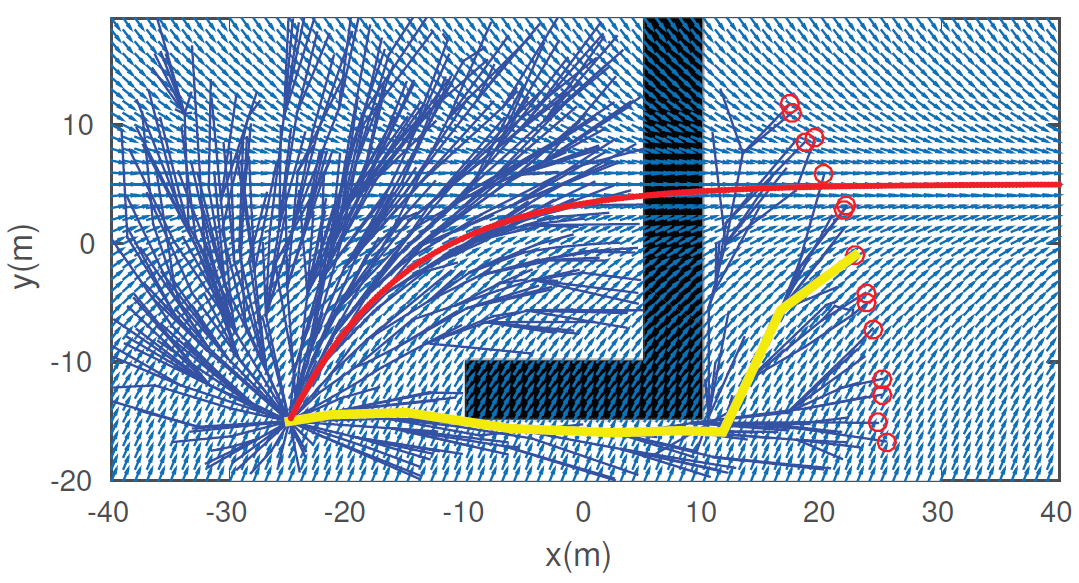
\includegraphics[width=12cm]{PaperFigures/rrtVF}
	\caption{RRT* path planner with a VF used as a task specification \cite{pereira_framework_2016}}
	\label{fig:rrtvf}
\end{figure}


Constrained Delaunay triangulation (CDT) has been used to generate an optimal path in an urban environment containing buildings \cite{md_simplex_2017}. CTD was used to construct vector fields in \cite{pimenta_fully_2007} that restricts robots movements inside the triangles while moving towards a global goal. A simulation of a robot traversing a vector field inside a set of CDTs can be seen in Figure \ref{fig:cdtVF}.

\begin{figure}
	\centering
	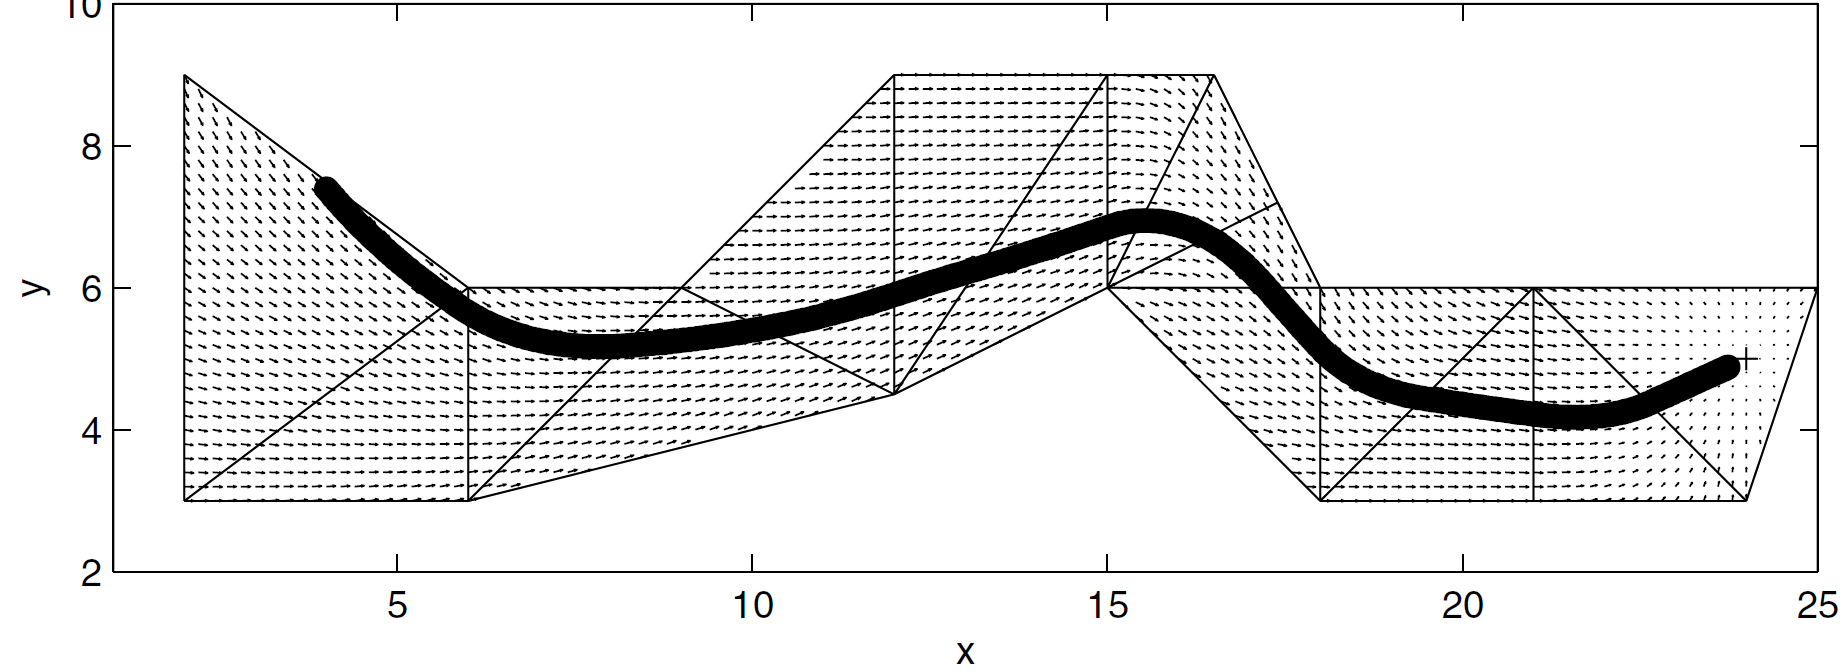
\includegraphics[width=15cm]{PaperFigures/cdtVF}
	\caption{Vector field within a set of constrained delaunay triangles \cite{pimenta_fully_2007}}
	\label{fig:cdtVF}
\end{figure}


So far all of the vector field methods discussed have avoided obstacles by planning paths around them. Paths are typically calculated at the ground station and if communication is lost a new path may not be relayed to a UAV encountering a new obstacle. A possible solution is using vector fields to provide a repulsive force, not unlike the VFF method, circumnavigating around the obstacle. 



% = = = = = = = = = = = = = = = = = = Think about using something like this in the literature review summary
%So far vector fields built from straight line and circular primitives that are commonly used by path planners to construct missions have been discussed. The method used to build primitives can be extended to construct vector fields that asymptotically converge to curved paths.  Primitives can be modified with coordinate transforms to construct racetrack and elliptical shapes for target following of moving and uncertain targets. Obstacles can be avoided through RRT* that uses a vector field to sense the general direction of branch expansion, and a robotic system can maintain a collision free path inside of a set of constrained triangles with vector fields.

\subsection{Gradient Vector Field}
Gradient vector field (GVF) is a method that produces an \textit{n}-dimensional vector field that converges and circulates a target path\cite{goncalves_artificial_2009}. Paths can be static or time-varying and consist of points that lie at the intersection of surfaces defined by implicit functions. The surface functions are used to calculate a total vector field that is a sum of a convergence, circulation, and time-varying term. Convergence effectively attracts a robot to the target curve while circulation guides the robot to traverse the target curve. Time-varying is a feed-forward term that accounts for changes in the target path as a function of time \textit{t}. The total field is summarized in Equation \ref{simpleGVF}.

\begin{equation}\label{simpleGVF}
\vec{v} = \vec{v}_{conv} + \vec{v}_{circ} + \vec{v}_{tv} 
\end{equation}

Multiplicative scalar weights (\textit{\textbf{G,H,L}}) have been used to modify the strength of each term in \cite{goncalves_circulation_2010}[wwc], shown in Equation \ref{weightedSimpleGVF}

\begin{equation}\label{weightedSimpleGVF}
\vec{v} = \boldsymbol{G}\vec{v}_{conv} + \boldsymbol{H}\vec{v}_{circ} + \boldsymbol{L}\vec{v}_{tv} 
\end{equation}


Producing a GVF that converges and circulates a target path consisting of points $\in$ $\mathbb{R}^n$, first requires \textit{(n-1)} implicit surface functions {$\alpha_i(x_1,x_2,...x_{n-1},t), i=1,2,...n-1$} to be defined. UAVs are restricted to $\mathbb{R}^3$ spatial configuration space, therefore two surface functions must be defined to calculate a GVF. Surface functions must have 1) \textit{continuous first order partial derivatives} and 2)\textit{ bounded second order partial derivatives} to guarantee convergence to the curve \cite{goncalves_circulation_2010}. The total gradient vector field converges and circulates the intersection, or level sets, of the two surfaces. For a UAV traveling at constant altitude, the first surface can be represented as a flat plane in Equation \ref{planeZ}. Intersecting the flat plane with a static vertical plane, Equation \ref{planeX}, produces a gradient vector field that converges and follows a straight line, Figure \ref{fig:gvfLinePrimitive}.

\begin{equation}
\label{planeZ}
\alpha_1 = z
\end{equation}

\begin{equation}
\label{planeX}
\alpha_2 = x
\end{equation}

\begin{figure}[H]
	\begin{subfigmatrix}{2}% number of columns
		\centering	
		\subfigure []{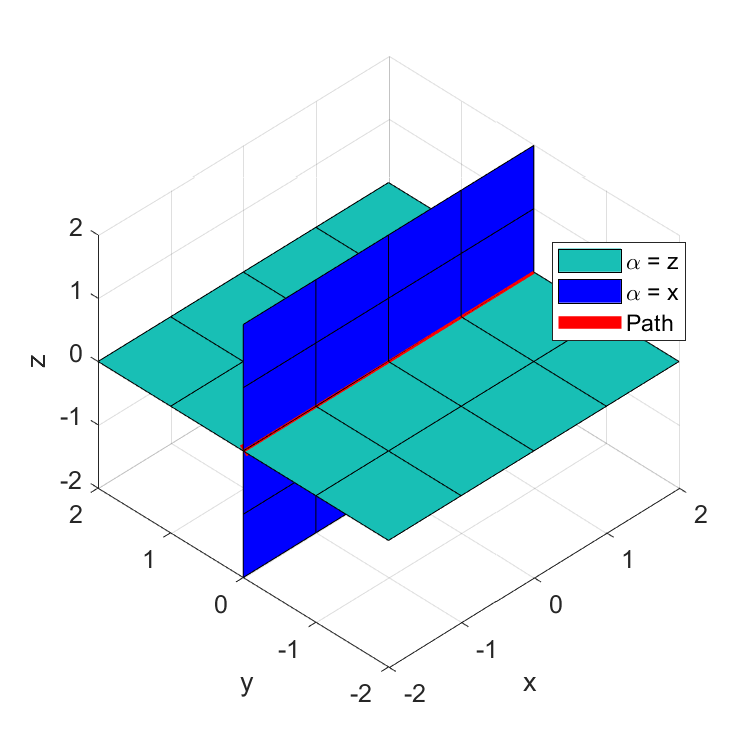
\includegraphics[width=7.5cm] {PaperFigures/planeIntersection}}
		\subfigure []{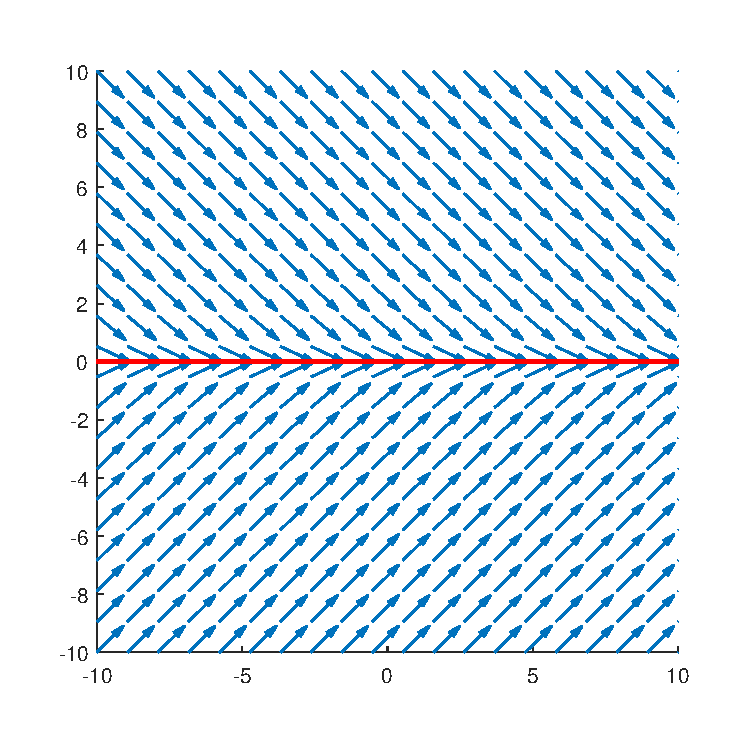
\includegraphics[width=7.5cm] {PaperFigures/compWithoutTitles/lineConvCirc}}
		\hspace*{0mm}
	\end{subfigmatrix}
	\caption{Intersection of planes (a) and resultant Gradient Vector Field (b)}
	\label{fig:gvfLinePrimitive}
\end{figure}

Similarly, intersecting the flat plane with a static cylinder, Equation \ref{cylinder}, results in a vector field that converges and follows a circular path shown in Figure \ref{fig:gvfCircPrimitive}.

\begin{equation}
\label{cylinder}
\alpha_2 = x^2+y^2-r^2
\end{equation}

\begin{figure}[H]
	\begin{subfigmatrix}{2}% number of columns
		\centering	
		\subfigure []{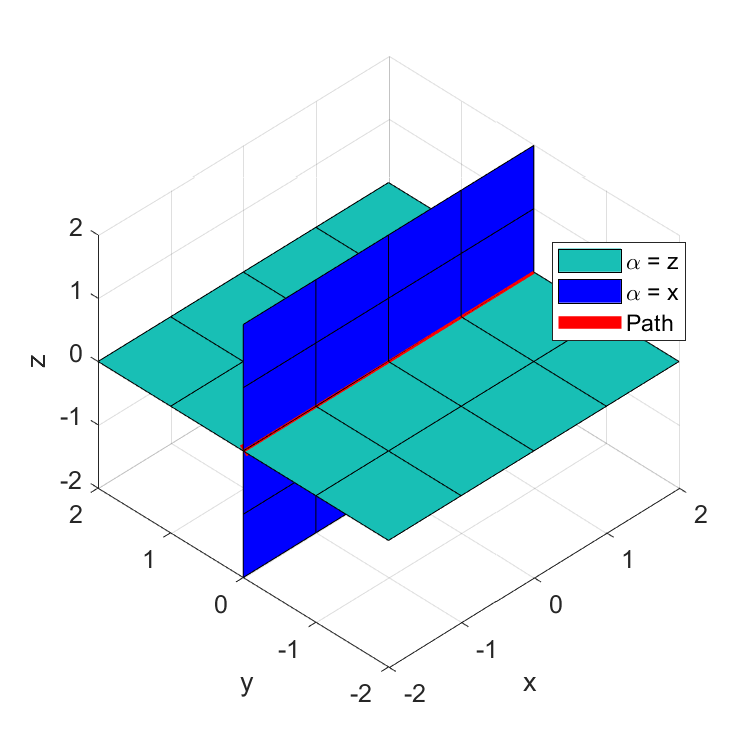
\includegraphics[width=7.5cm] {PaperFigures/planeIntersection}}
		\subfigure []{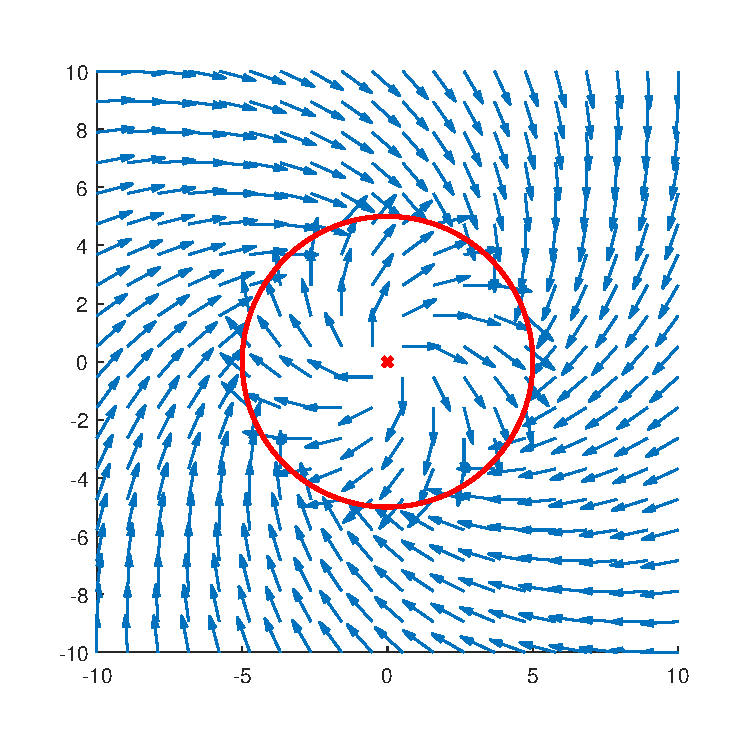
\includegraphics[width=7.5cm] {PaperFigures/compWithoutTitles/circConvCirc}}
		\hspace*{0mm}
	\end{subfigmatrix}
	\caption{Intersection of plane / cylinder (a) and resultant Gradient Vector Field (b)}
	\label{fig:gvfCircPrimitive}
\end{figure}

Static paths do not require the time-varying term of the vector field calculation and can be considered zero in such cases. The convergence term of the vector field is calculated by summing the product of each implicit function with its own gradient, which is shown in Equation \ref{convOnly}.

\begin{equation}
% Total field with Conv, Circ, and Time
\vec{v}_{conv} = \sum_{i=1}^{n-1}\alpha_i\nabla_q\alpha_i  
\label{convOnly}
\end{equation}


Evaluating equation \ref{convOnly} for a cylinder intersecting a plane results in a vector field that converges to a circular path shown in Figure \ref{fig:gvfCircAttractive}a. Note that the vectors are not of equal length for the entire configuration space, decaying in strength when approaching the curve. Normalizing the field was done in [wwc] \cite{goncalves_circulation_2010,goncalves_vector_2010} to allow for convenient weighting of each term at a later process. The normalized convergence field for a circular path is shown in Figure \ref{fig:gvfCircAttractive}b. 

\begin{figure}[H]
	\begin{subfigmatrix}{2}% number of columns
		\centering	
		\subfigure []{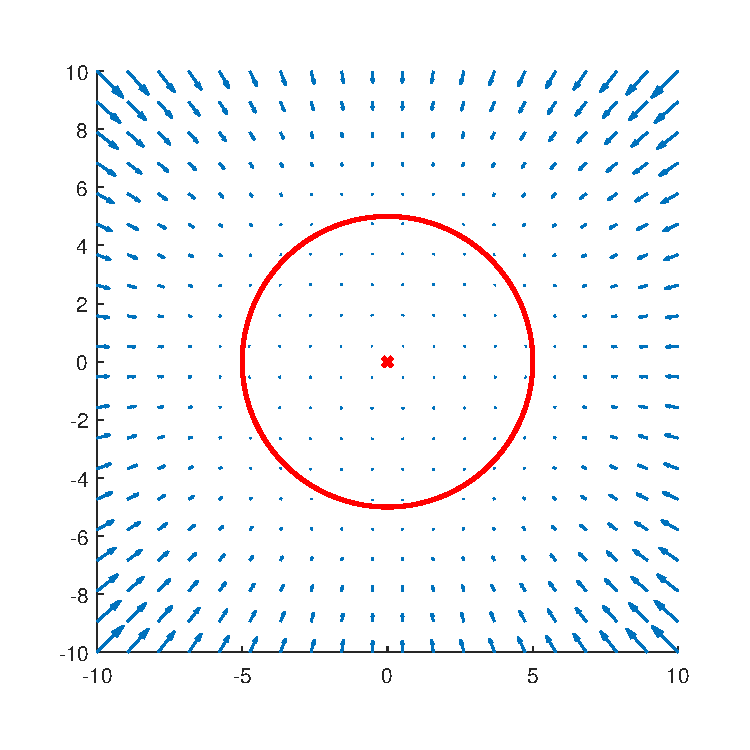
\includegraphics[width=7.5cm] {PaperFigures/NNcompWithoutTitles/circAttractive}}
		\subfigure []{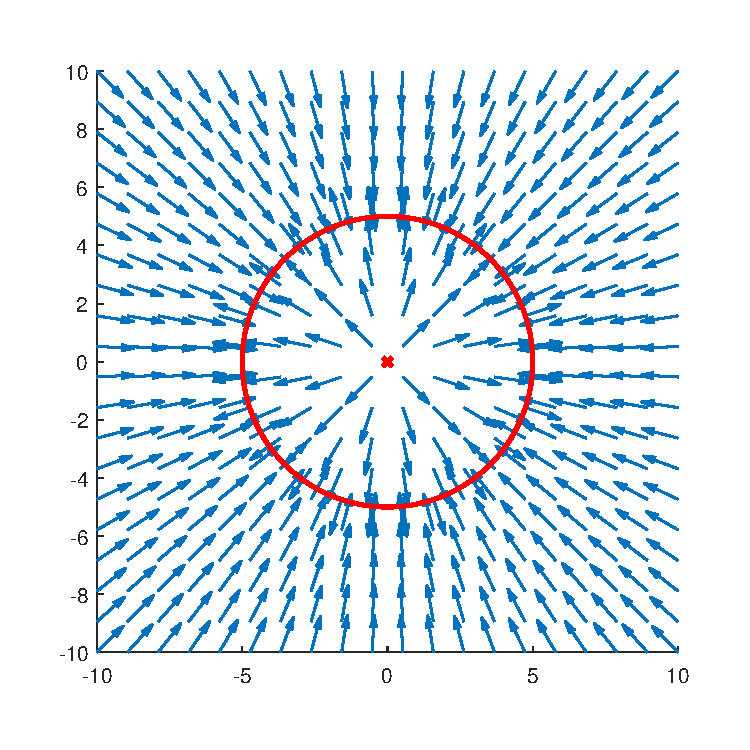
\includegraphics[width=7.5cm] {PaperFigures/compWithoutTitles/circAttractive}}
		\hspace*{0mm}
	\end{subfigmatrix}
	\caption{GVF circular attractive field without normalization (a) and with normalization (b)}
	\label{fig:gvfCircAttractive}
\end{figure}

The circulation term is calculated by taking the wedge product of each surface's gradient, shown in Equation \ref{circOnly}. For surfaces in $\mathbb{R}^3$, the wedge product can be simplified to the cross product shown in Equation \ref{circOnlySimp}.

\begin{equation}
% Total field with Conv, Circ, and Time
\vec{v}_{circ} =  \wedge_{i=1}^{n-1}\nabla_q\alpha_i 
\label{circOnly}
\end{equation}

\begin{equation}
% Total field with Conv, Circ, and Time
\vec{v}_{circ} =  \nabla_q\alpha_1 \times \nabla_q\alpha_2 
\label{circOnlySimp}
\end{equation}


Evaluating the circulation term results in a vector field that is parallel to a circular path, shown in Figure \ref{fig:gvfCircCirculation}a. The field is normalized to produce a field with equal length vectors for the configuration space which is shown in Figure \ref{fig:gvfCircCirculation}b. 

\begin{figure}[H]
	\begin{subfigmatrix}{2}% number of columns
		\centering	
		\subfigure []{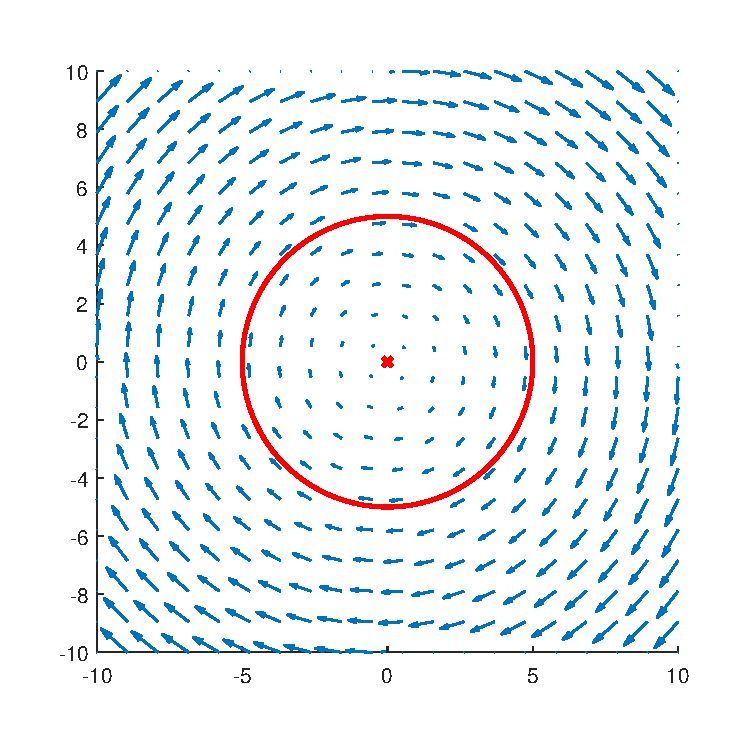
\includegraphics[width=7.5cm] {PaperFigures/NNcompWithoutTitles/circCW}}
		\subfigure []{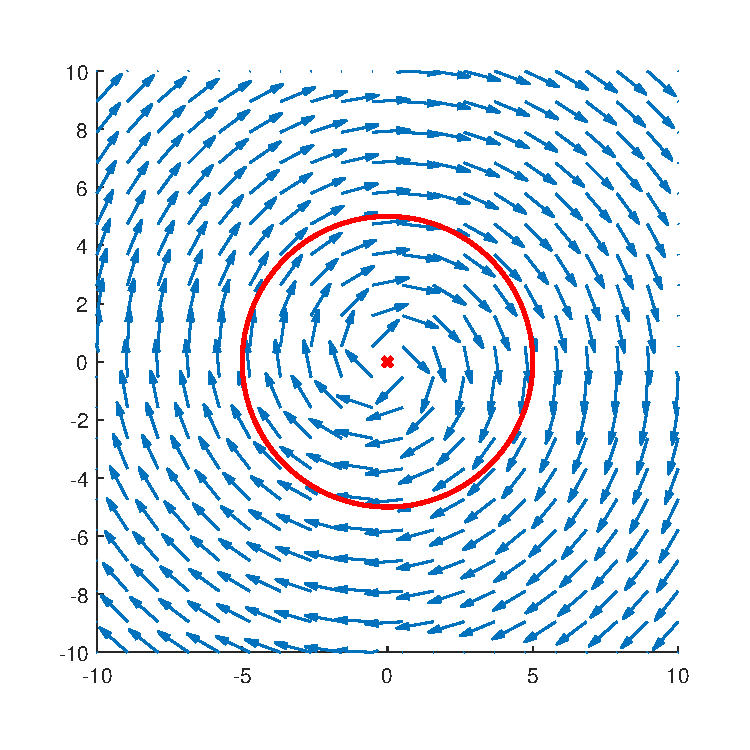
\includegraphics[width=7.5cm] {PaperFigures/compWithoutTitles/circCW}}
		\hspace*{0mm}
	\end{subfigmatrix}
	\caption{Circular GVF without normalization (a) and with normalization (b)}
	\label{fig:gvfCircCirculation}
\end{figure}

For dynamic paths that vary in time \textit{t}, feedforward compensation is accomplished by calculating the time-varying term. The time-varying field is calculated by multiplying the inverse of the gradient matrix $M$ with the column vector $a$ shown in Equations \ref{mMatrix} and \ref{aVector} respectively. The resulting vector field for a circular path moving in the positive x direction can be shown in Figure \ref{fig:gvfCircTimeVarying}a and the normalized version in Figure \ref{fig:gvfCircTimeVarying}b.


\begin{equation}
\label{mMatrix}
M =\begin{bmatrix}
\nabla\alpha_1^T \\
\nabla\alpha_2^T \\
(\nabla\alpha_1 \times \nabla\alpha_2)^T
\end{bmatrix}
\end{equation}

\begin{equation}
\label{aVector}
a =\begin{bmatrix}
\frac{\partial \alpha_1}{\partial t} \quad   \frac{\partial \alpha_2}{\partial t} \quad   0
\end{bmatrix}^T
\end{equation}


\begin{figure}[H]
	\begin{subfigmatrix}{2}% number of columns
		\centering	
		\subfigure []{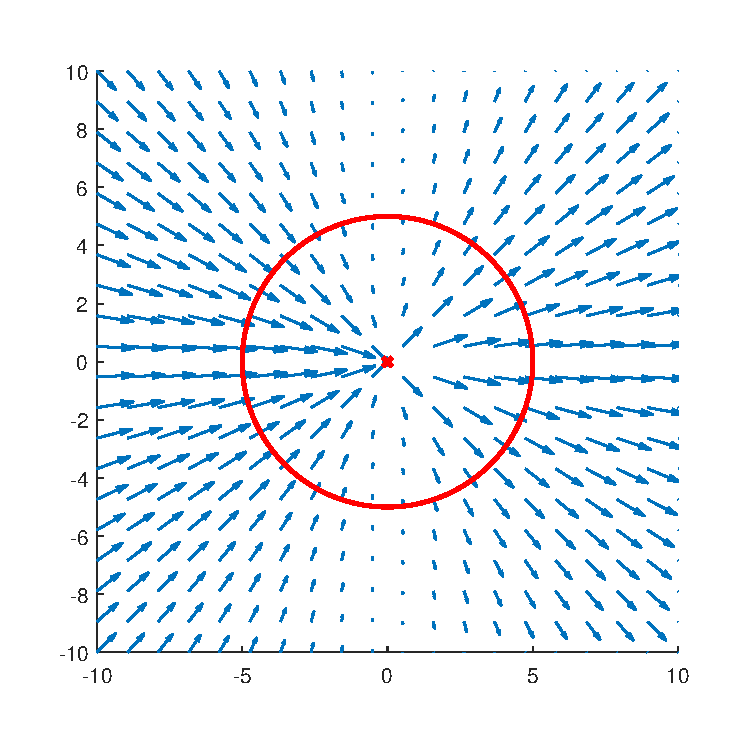
\includegraphics[width=7.5cm] {PaperFigures/NNcompWithoutTitles/circTv}}
		\subfigure []{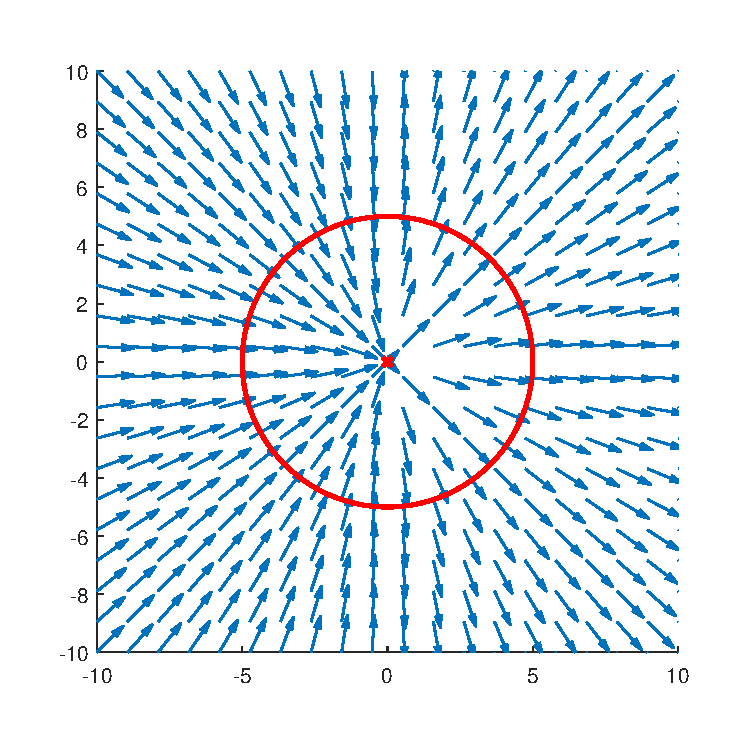
\includegraphics[width=7.5cm] {PaperFigures/compWithoutTitles/circTv}}
		\hspace*{0mm}
	\end{subfigmatrix}
	\caption{Circular time-varying GVF without normalization (a) and with normalization (b)}
	\label{fig:gvfCircTimeVarying}
\end{figure}

Summing together the normalized convergence, circulation, and time-varying terms results in the total field $\vec{V}$ shown defined in Equation \ref{gonAllComp}. Scalar weights, (\textit{\textbf{G,H,L}}), are added after normalization to increase or decrease the contribution of convergence, circulation, and time-varying respectively. 

\begin{equation}
% Component vector field with conv and circ
\vec{V} = \boldsymbol{G}||\vec{v}_{conv}|| + \boldsymbol{H}||\vec{v}_{circ}|| +  \boldsymbol{L}||\vec{v}_{tv}|| 
\label{gonAllComp}
\end{equation}


\begin{figure}
	\centering
	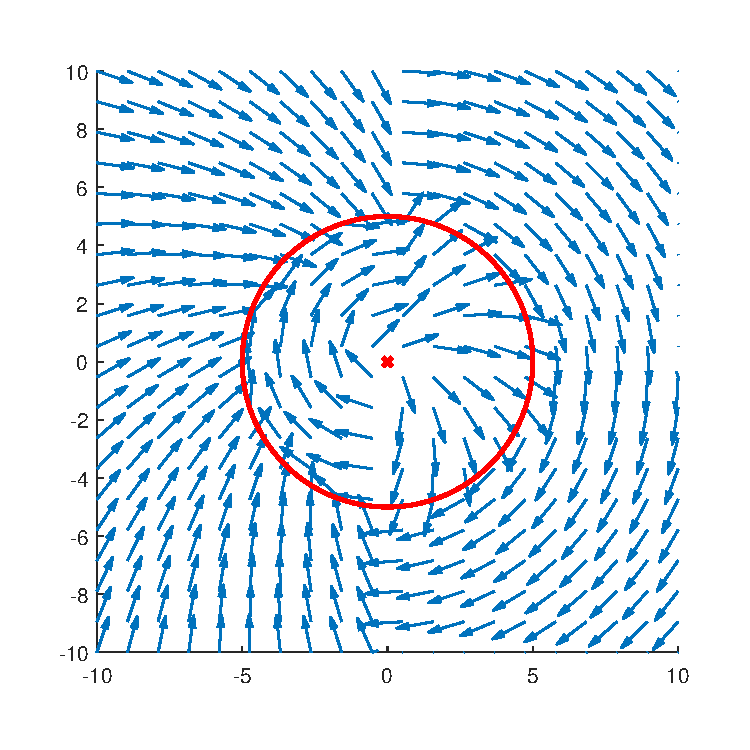
\includegraphics[width=8cm]{PaperFigures/compWithoutTitles/circConvCircTv}
	\caption{GVF with unity (\textit{\textbf{G=H=L=1}}) weights for a moving circular path}
	\label{fig:circconvcirctv}
\end{figure}

The GVF weights are decoupled from each term calculation, therefore modifications to the GVF weights do not require a new derivation of the resulting field. Magnitude of the weights effectively scales the contribution of each term. Negating the GVF weights has been used to provide a repulsive field for obstacle avoidance in [wwc] for a UAV tracking a moving loiter circle. Assigning weights \textbf{G=-1} and \textbf{H=L=0} rotates the attractive field vectors in Figure \ref{fig:gvfCircAttractive}b 180$^\circ$ about the tail of each vector, which is shown in Figure \ref{fig:gvfRepulsiveRadius}a. Note how the repulsive field vectors point away from the circular curve for the entire configuration space. Encircling an obstacle by a path produces vectors that may provide guidance into the obstacle, which is not desired. Reducing the radius to be smaller than the radius of the obstacle produces a GVF with nearly all vectors directing away. 


\begin{figure}[H]
	\begin{subfigmatrix}{2}% number of columns
		\centering	
		\subfigure []{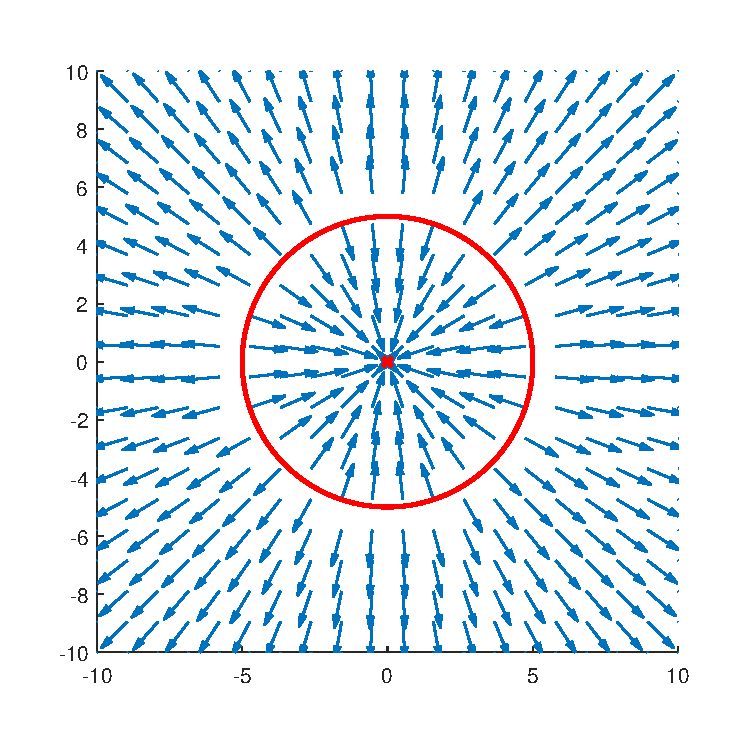
\includegraphics[width=6.5cm] {PaperFigures/compWithoutTitles/circRepulsive}}
		\subfigure []{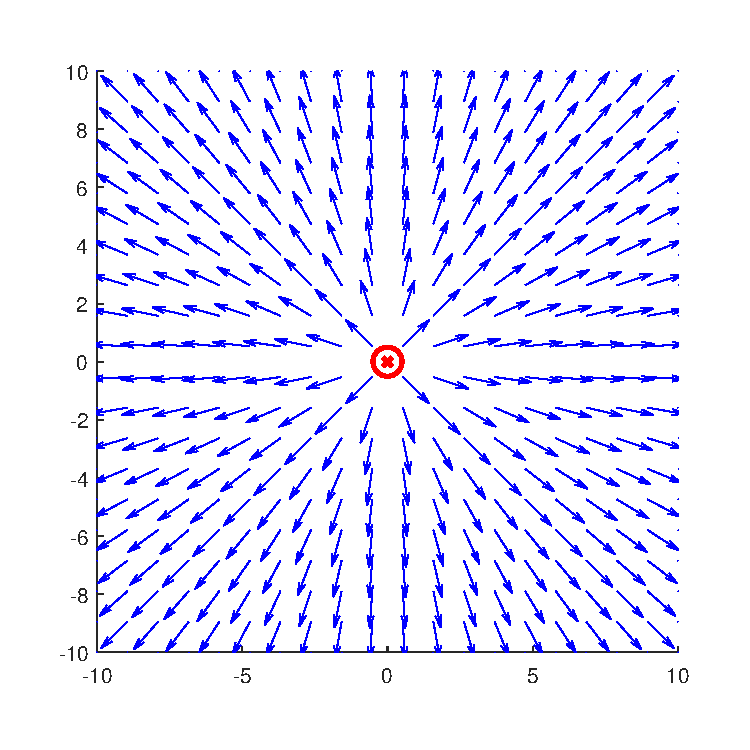
\includegraphics[width=6.5cm] {PaperFigures/compWithoutTitles/circRepulsiveSmallr}}
		\hspace*{0mm}
	\end{subfigmatrix}
	\caption{Repulsive field with large path radius (a) and small radius (b)}
	\label{fig:gvfRepulsiveRadius}
\end{figure}

The strength of the repulsive field was varied as a function of proximity $d$ by multiplying the repulsive field by a decay function $P$ bounded on the interval [-1,0], shown in Equation \ref{repulsiveDecay} and Figure \ref{fig:tanhICUAS2018}. The radius $R$ is the distance from the center of the field where vectors have effectively zero strength. 

\begin{equation}
P = R\frac{tanh(2\pi d-\pi)+1}{2}
\label{repulsiveDecay}
\end{equation}

\begin{equation}
\vec{v}_{repulsive} = -G||\vec{v_{conv}}||P
\label{replulsiveField}
\end{equation}



\begin{figure}[H]
	\begin{subfigmatrix}{2}% number of columns
		\centering	
		\subfigure []{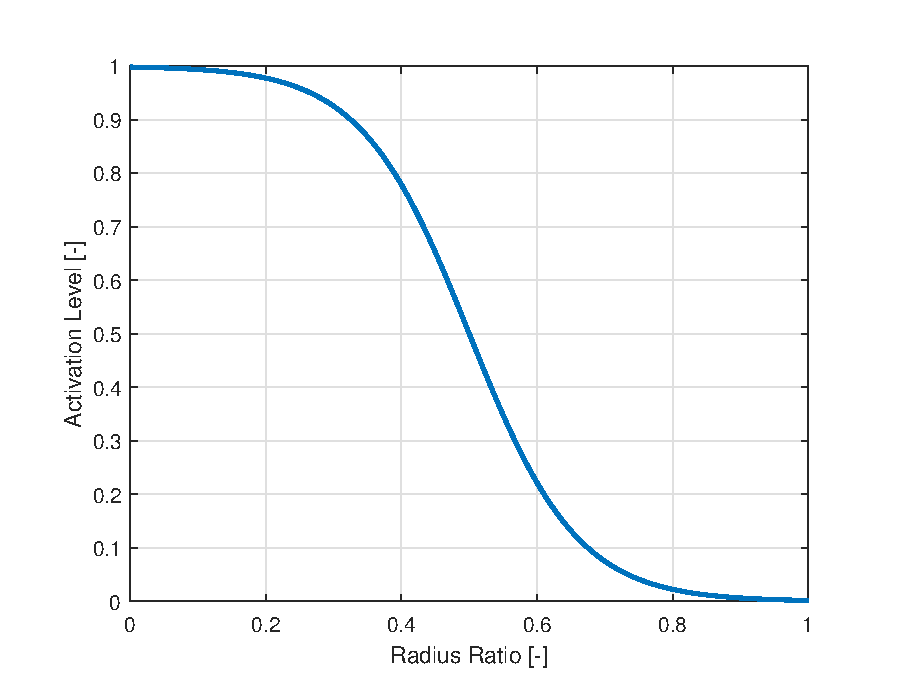
\includegraphics[width=8cm] {PaperFigures/tanh_ICUAS2018}}
		\subfigure []{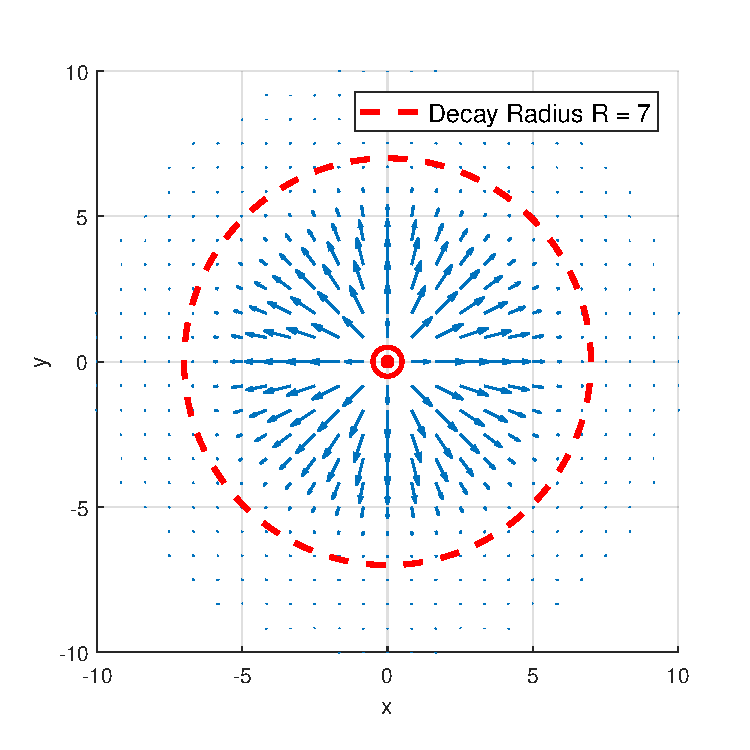
\includegraphics[width=7cm] {PaperFigures/repulsiveFields/circRepulsiveDecay}}
		\hspace*{0mm}
	\end{subfigmatrix}
	\caption{Repulsive field activation [wwc](a) resulting repulsive field (b)}
	\label{fig:tanhICUAS2018}
\end{figure}


Attractive and repulsive fields were added together and the resulting vector shown in Equation \ref{summedAttRepulsive}. The resultant heading vector was used to guide a UAV to track a moving loiter circle while avoiding static obstacles, shown in Figure \ref{fig:gvfMovingTarget}.

\begin{equation}
\vec{V} = \vec{v}_{attractive}+\vec{v}_{repulsive}
\label{summedAttRepulsive}
\end{equation}



\begin{figure}[h]
	\centering
	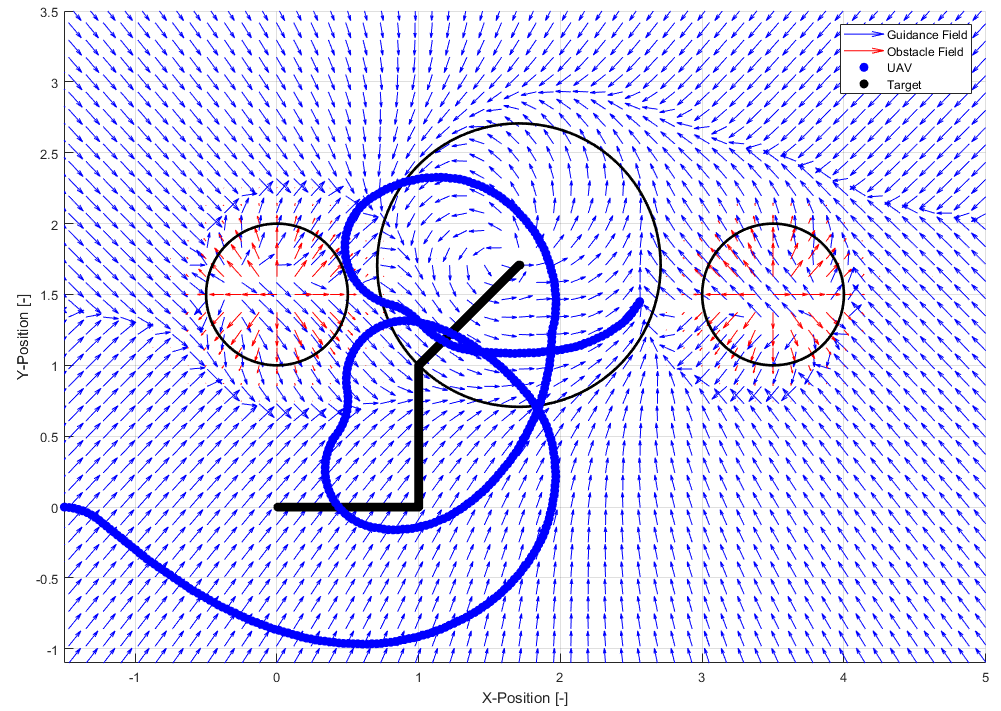
\includegraphics[width=10cm]{PaperFigures/gvfMovingTarget}
	\caption{Place holder image of UAV following ground target [wwc]}
	\label{fig:gvfMovingTarget}
\end{figure}


GVF weights have been used for high level specification of the desired behavior for a UAV, whether it be for convergence, circulation, or avoidance. Repulsive GVFs have considered obstacle fields that strictly repel. The strictly repulsive guidance is effective at directing a UAV away from an obstacle, but provides no information on how to circumnavigate one. Additionally, further specification on the minimum radius and strength of the repulsive field may be useful in preventing a UAV from violating the obstacle circle. A preliminary simulation shows that a UAV encountering an obstacle while tracking a path may result in violation of the obstacle space, shown in Figure \ref{fig:singleobstacle}. UAVs traveling at lower velocities
 may also enter a trap situation where the guidance is confined to an infinite loop.
 \pagebreak

\begin{figure}[h]
	\centering
	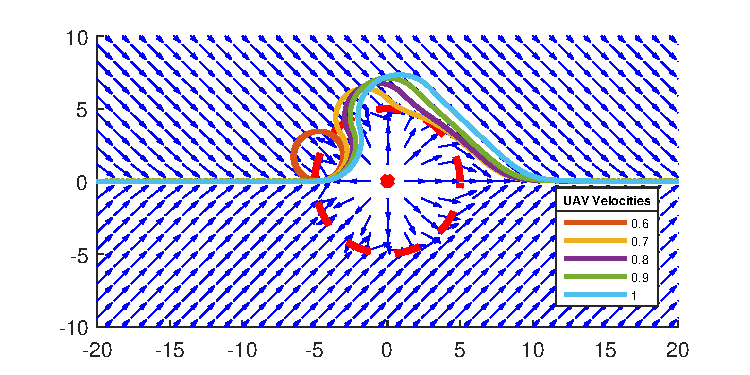
\includegraphics[width=12cm]{PaperFigures/singleObstacle}
	\caption{}
	\label{fig:singleobstacle}
\end{figure}


Adding circulation \textit{\textbf{H=1}} to the GVF in Figure \ref{fig:singleobstacle} prevented the trap situation for a velocity $v = 0.6$ and reduced the circumnavigation distance, which is shown in Figure \ref{fig:singleobstacleWithCirc}. Specifying vector field weights as functions of a UAV's state may enable an optimal guidance for obstacle avoidance. 

\begin{figure}[h]
	\centering
	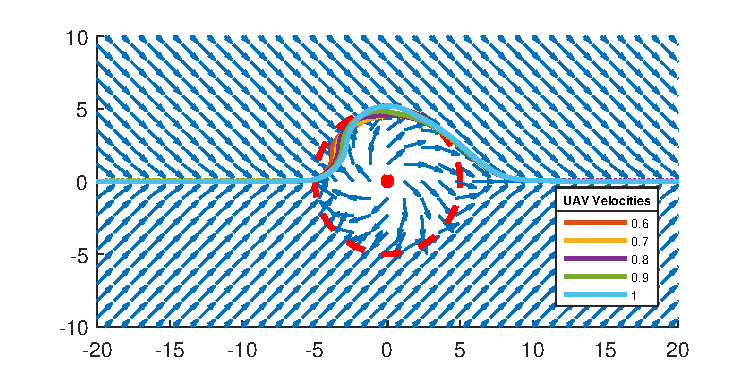
\includegraphics[width=12cm]{PaperFigures/singleObstacleWithCirc}
	\caption{}
	\label{fig:singleobstacleWithCirc}
\end{figure}




\pagebreak
\section{Unmanned Aerial Vehicle Simulation}
Testing new guidance, navigation, and control algorithms on flight hardware can be costly, require significant time, and requires an adequately large airspace. Before spending the time to reserve airspace and allocate man hours for flight tests it is important to test algorithms in a controlled environment. One way to accomplish testing without actual flight is through validation through mobile robots simulating fixed wing constraints \cite{ren_experimental_2007}, \cite{louali_designing_2014}, \cite{louali_experimental_2016}. Programming a mobile robot, such as one shown in Figure \ref{fig:robot}.

\begin{figure}
	\centering
	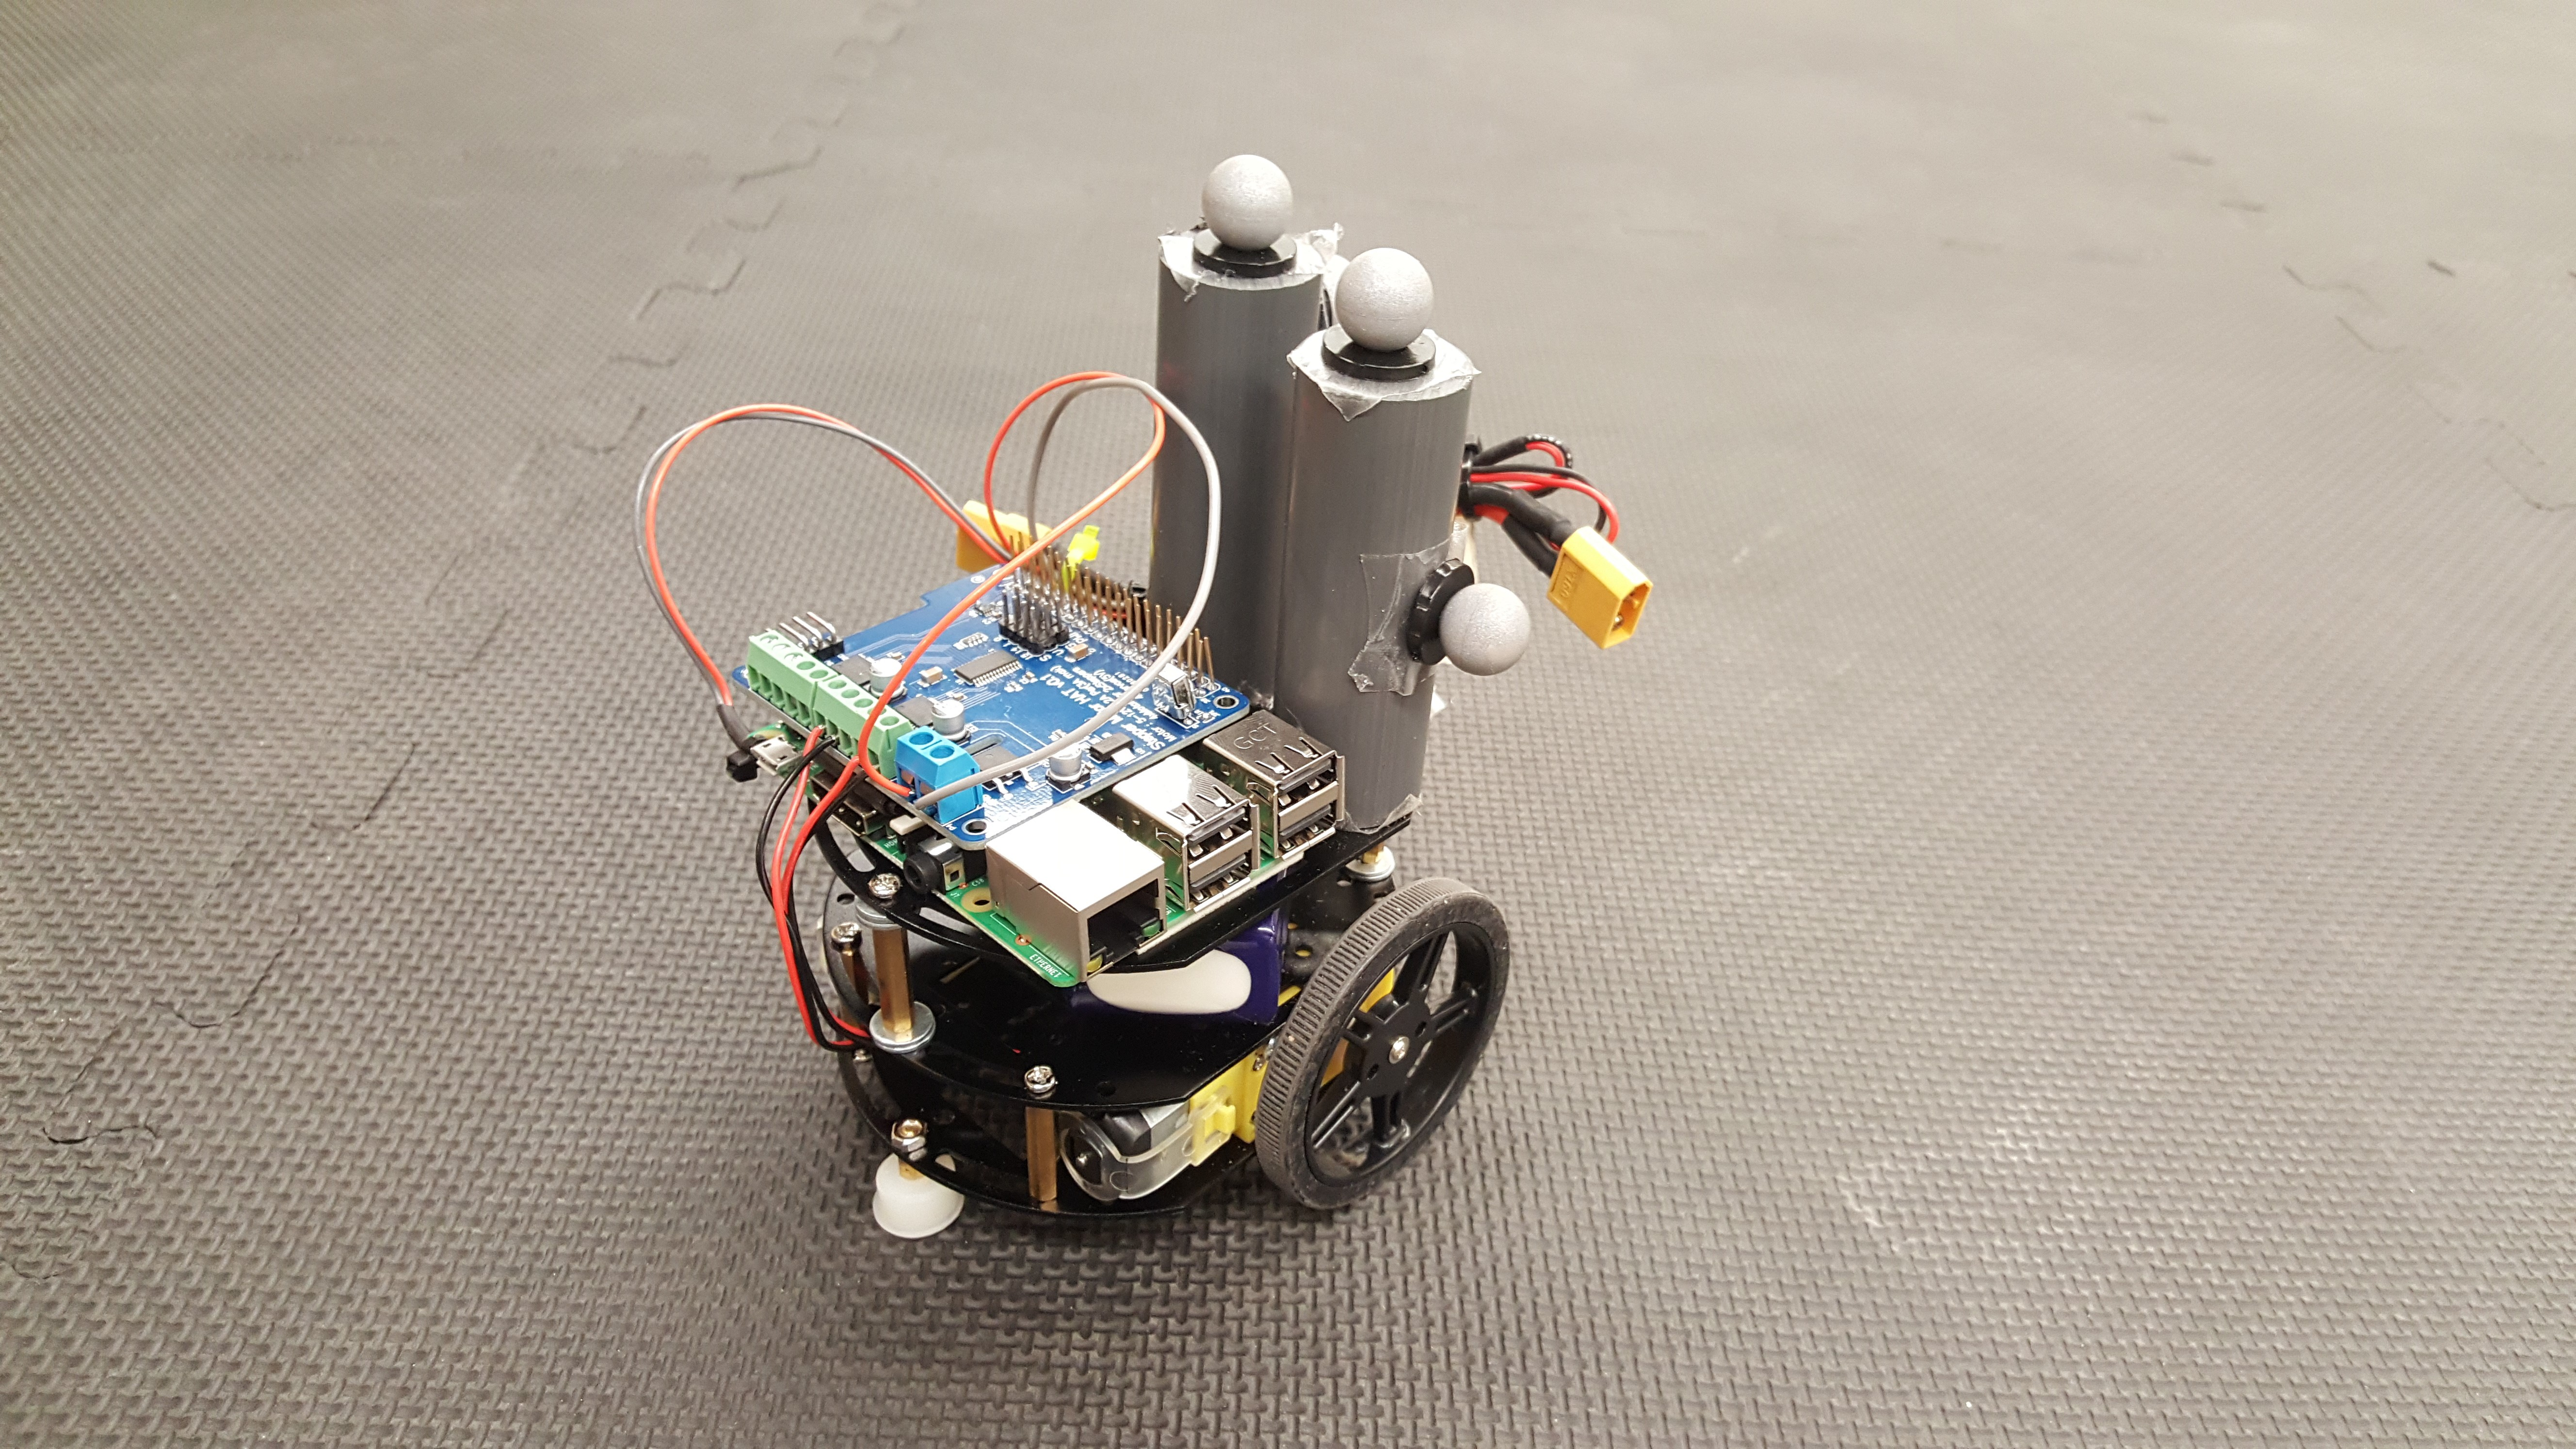
\includegraphics[width=15cm]{PaperFigures/robot}
	\caption{Differential drive mobile robot simulating fixed wing UAV Dubins constraints}
	\label{fig:robot}
\end{figure}


\section{Literature Review Summary}


Vector fields can provide guidance and control for robots through the use of artificial attractive and repulsive forces. Converging to a singular point while avoiding obstacles can be achieved with Potential Field or Virtual Force Field methods. Fixed wing UAVs cannot converge to a singular point therefore vector fields that asymptotically converge and follow a path is beneficial. Lyapunov and Gradient Vector Fields have been used for path following, standoff tracking, and obstacle avoidance. Gradient Vector Field provides convenient and decoupled access to scalar multiplicative weights for the convergence, circulation, and time-varying terms. Negative weights can be used for obstacle avoidance, however have so far been used only as high level specification of guidance behavior. Specifying vector field weights as functions of a UAV's state may enable an optimal guidance for obstacle avoidance. Validation of a modified GVF guidance can be performed on mobile ground robots simulating UAV dynamics.

\chapter{Methodology}
\section{Methods Overview}
The proposed research will be conducted in three phases where VF guidance  singularities will be demonstrated, weighting functions will be investigated, and a developed GVF will be validated on a ground robot simulating a UAV.  Phases I and II will be conducted in a simulation environment that combines mission paths and obstacles into a single GVF. Phase III will be conducted with a ground robot simulating a UAV guided by the modified GVF in real-time. Dubin's fixed wing constraints will be imposed in simulations and experiments. 


\section{Phase I}
\textbf{Demonstrate GVF singularities for circular obstacles.} A simulation environment will be built that generates GVFs consisting of mission paths and obstacles. Circular and elliptical obstacles will be investigated and the resulting singularities will be characterized. Static weights will be used and the performance of the guidance measured in distance traveled and time of flight. 



\section{Phase II}
\textbf{Investigate GVF weighting functions that influence obstacle avoidance.} UAV closing rate, position, and range will be used to develop dynamic GVF weights for convergence and circulation. The modified GVF will be compared against a static and strictly repulsive GVF. Distance traveled and time of flight will be used to as metrics to compare the modified GVF to the unmodified GVF.  



\section{Phase III}
\textbf{Validate modified GVF model with ground robot experiments.} The modified GVF developed in Phase II will be implemented on a differential drive ground robot simulating a fixed wing UAV. Guidance performance while avoiding static obstacles will be demonstrated.


\section{Summary of Phases}

Each phase consists of an \textbf{objective} that will be accomplished by executing \textit{tasks}.
Completion of all objectives and phases will result in the final \underline{deliverable}. \\[1cm]

\noindent
\textbf{Phase I:} Demonstrate Gradient Vector Field Singularities
\textit{
	\begin{enumerate}
		\item Build a GVF simulation environment
		\item Derive GVF for circular and elliptical obstacles
		\item Identify path and obstacles where singularities are produced 
	\end{enumerate}
}

\noindent
\textbf{Phase II:} Investigate GVF weighting functions that influence obstacle avoidance
\textit{
	\begin{enumerate}
		\item Formulate circulation and convergence weights as functions of UAV state
		\item Determine combination of GVF weights that produces optimal guidance in simulation
	\end{enumerate}
}

\noindent
\textbf{Phase III:} Validate modified GVF model with ground robot experiments
\textit{
	\begin{enumerate}
		\item Build differential drive robot
		\item Build robotic framework to take guidance commands
		\item Repeat simulations performed in Phase II on ground robot
	\end{enumerate}
}

\noindent
\textbf{Deliverable:} \underline{Adaptive GVF parameterized weights optimal guidance for path following and static} \underline{ obstacle avoidance}.



\bibliographystyle{aiaa}   
\bibliography{bib}


\end{document}
